						%Bachelorarbeit 2020 Julian Leupold
%___________________________________________________%

\documentclass[12pt, a4paper, listof=totoc, parskip=half, bibliography=totoc, abstract=on]{scrbook} %documentclass
\usepackage{verbatim} %comments for more than one line
%\renewcommand{\familydefault}{\ttdefault} %%change font
%---% to use utf-8 as input codec
\usepackage{ucs} 
\usepackage[utf8x]{inputenc}
\usepackage{paralist} %%use compactintemize
\usepackage{pdflscape} %%to rotate some sites
%---%
\usepackage[onehalfspacing]{setspace} %to modify line spacing
\usepackage[T1]{fontenc} %to use "umlaute", textcodec
\usepackage[ngerman]{babel} %to use german as doc language
\usepackage{amsmath,amssymb,amstext} %to use math display
\usepackage{float} %use of floating objects (graphics, tables, ..)
\usepackage{flafter} %prevents float to appear before their definition
\usepackage[automark, headsepline]{scrpage2} %heatseperationline
\usepackage[footnote]{acronym} %make acronyms as footnotes
\usepackage{color,soul} %to highlight text
\usepackage{relsize} %to set font sizes relative to current sizes
\usepackage{graphicx} %to include pdfs
\usepackage{pdfpages} %to incluzde pdfs
\usepackage{tocloft} %to modify toc for supressing pagenumbers
\renewcaptionname{ngerman}{\abstractname}{Abstract} %to include abstracts
\renewcommand{\chapterheadstartvskip}{\vspace{0.1cm}} %remove space before chapter
\usepackage[section]{placeins}
%
%----------------------------------------------------% to highlight hyperlinks different
\usepackage[
    bookmarks,
    bookmarksopen=true,
    colorlinks=true,
% diese Farbdefinitionen zeichnen Links im PDF farblich aus
    %linkcolor=red, % einfache interne Verknüpfungen
    %anchorcolor=black,% Ankertext
    %citecolor=blue, % Verweise auf Literaturverzeichniseinträge im Text
    %filecolor=magenta, % Verknüpfungen, die lokale Dateien öffnen
    %menucolor=red, % Acrobat-Menüpunkte
    %urlcolor=cyan, 
% diese Farbdefinitionen sollten für den Druck verwendet werden (alles schwarz)
    linkcolor=black, % einfache interne Verknüpfungen
    anchorcolor=black, % Ankertext
    citecolor=black, % Verweise auf Literaturverzeichniseinträge im Text
    filecolor=black, % Verknüpfungen, die lokale Dateien öffnen
    menucolor=black, % Acrobat-Menüpunkte
    urlcolor=black, 
    backref,
    plainpages=false, % zur korrekten Erstellung der Bookmarks
    pdfpagelabels, % zur korrekten Erstellung der Bookmarks
    hypertexnames=false, % zur korrekten Erstellung der Bookmarks
    linktocpage % Seitenzahlen anstatt Text im Inhaltsverzeichnis verlinken
]{hyperref}
%------------------------------------------------------------%
\usepackage{textcomp} %provide textsymbols
% zum Einbinden von Programmcode -----------------------------------------------
\usepackage{listings}
\usepackage{color}
\definecolor{hellgelb}{rgb}{1,1,0.9}
\definecolor{colKeys}{rgb}{0,0,1}
\definecolor{colIdentifier}{rgb}{0,0,0}
\definecolor{colComments}{rgb}{1,0,0}
\definecolor{colString}{rgb}{0,0.5,0}
%\lstset{
%	tabsize=3,
%	extendedchars=true,
%	frame=single,
%	showstringspaces=true,
%	numbers=left,
%	numberstyle=\small,
%	breakautoindent=true,
%	breaklines=true,
%    postbreak=\mbox{\textcolor{red}{$\hookrightarrow$}\space},
%    showstringspaces=false,
%} 
\lstset{
    float=hbp,
    basicstyle=\ttfamily\color{black}\small\smaller,
    identifierstyle=\color{colIdentifier},
    keywordstyle=\color{colKeys},
    stringstyle=\color{colString},
    commentstyle=\color{colComments},
    columns=flexible,
    tabsize=2,
    frame=single,
    extendedchars=true,
    showspaces=false,
    showstringspaces=false,
    numbers=left,
    numberstyle=\tiny,
    breaklines=true,
    backgroundcolor=\color{hellgelb},
    breakautoindent=true
} 

%------------------------------------------------
\usepackage[gen]{eurosym} %eurosymbol
\usepackage{geometry} %to adjust page geometry
\usepackage{svg} %to import svg graphics

% Hurenkinder und Schusterjungen verhindern
\clubpenalty10000
\widowpenalty10000
\displaywidowpenalty=10000
%----%

%% counter for appendix stuff, not used atm
%\newcounter{savesection}
%\newcounter{apdxsection}

\setcounter{tocdepth}{1} % the last shown points in the toc are sections


% my own sitelayout
\pagestyle{scrheadings}
\clearscrheadfoot
\cfoot[]{\writer}
\ofoot[\pagemark]{\pagemark} 
\ihead[]{
\includegraphics[height=30pt]{Bilder/th.jpg}} 
\ohead[]{
\includegraphics[height=35pt]{Bilder/siemenslogo.png}}
\addtolength{\headsep}{\baselineskip}
%
%
% start of document
%% all the pagesize stuff was testing/layouting, maybe need for it again
%command for posting pictures at the spot, where they are defined
%#1 name of picture
%#2 width of picture as part of textwidth (height will scale automattically)
%#3 caption of the picture
%#4  label or references
%call -> \bild{#1}{#2}{#3}{#4}
\newcommand{\pic}[4] 
{ 
   \begin{figure}[H]
   \begin{center}
   \includegraphics[width=#2\textwidth]{Bilder/#1} 
   \caption{#3} 
   \label{fig:#4} 
   \end{center}
   \end{figure} 
} 

%%quotationmarks
\newcommand{\markss}[1]
{
\glqq #1\grqq
}


%%% hab hier was mit appendix versucht, wird aber denke nicht benötigt
%\makeatletter
%\renewcommand\appendix{\par
 % \setcounter{savesection}{\value{section}}%
  %\setcounter{section}{\value{apdxsection}}%
  %\setcounter{subsection}{0}%
  %\gdef\thesection{\@Alph\c@section}}
  
%\newcommand\unappendix{\par
 % \setcounter{apdxsection}{\value{section}}%
 % \setcounter{section}{\value{savesection}}%
  %\setcounter{subsection}{0}%
  %\gdef\thesection{\@arabic\c@section}}
  
%\makeatother%

\newcommand{\inline}[1]
{
{\lstinline[language=C++,basicstyle=\ttfamily]!#1!} 
}
\newcommand{\matrikelnr}{3000866}
\newcommand{\location}{Erlangen}
\newcommand{\writer}{Julian Leupold}
\newcommand{\thisyear}{2020}
\newcommand{\fexaminer}{Prof. Dr. Joerg Arndt}
\newcommand{\sexaminer}{Prof. Dr. Helmut Herold}
\newcommand{\personofsupport}{Hr. Paul-Heinz Esters}
%% Anpassung des Seitenlayouts --------------------------------------------------
%   siehe Seitenstil.tex
% ------------------------------------------------------------------------------
\usepackage[
    automark, % Kapitelangaben in Kopfzeile automatisch erstellen
    headsepline, % Trennlinie unter Kopfzeile
    ilines % Trennlinie linksbündig ausrichten
]{scrpage2}

% Anpassung an Landessprache ---------------------------------------------------
\usepackage[ngerman]{babel}

% Umlaute ----------------------------------------------------------------------
%   Umlaute/Sonderzeichen wie aöüß direkt im Quelltext verwenden (CodePage).
%   Erlaubt automatische Trennung von Worten mit Umlauten.
% ------------------------------------------------------------------------------
\usepackage[utf8]{inputenc}
\usepackage[T1]{fontenc}
\usepackage{textcomp} % Euro-Zeichen etc.

% Schrift ----------------------------------------------------------------------
\usepackage{lmodern} % bessere Fonts
\usepackage{relsize} % Schriftgröße relativ festlegen

%Mehrseitige Tabellen
\usepackage{longtable}

% Grafiken ---------------------------------------------------------------------
% Einbinden von JPG-Grafiken ermöglichen
\usepackage[dvips,final]{graphicx}
% hier liegen die Bilder des Dokuments
\graphicspath{{Bilder/}}

% Befehle aus AMSTeX für mathematische Symbole z.B. \boldsymbol \mathbb --------
\usepackage{amsmath,amsfonts}

% für Index-Ausgabe mit \printindex --------------------------------------------
\usepackage{makeidx}

% Einfache Definition der Zeilenabstände und Seitenränder etc. -----------------
\usepackage{setspace}
\usepackage{geometry}

% Symbolverzeichnis ------------------------------------------------------------
%   Symbolverzeichnisse bequem erstellen. Beruht auf MakeIndex:
%     makeindex.exe %Name%.nlo -s nomencl.ist -o %Name%.nls
%   erzeugt dann das Verzeichnis. Dieser Befehl kann z.B. im TeXnicCenter
%   als Postprozessor eingetragen werden, damit er nicht ständig manuell
%   ausgeführt werden muss.
%   Die Definitionen sind ausgegliedert in die Datei "Glossar.tex".
% ------------------------------------------------------------------------------
\usepackage[intoc]{nomencl}
\let\abbrev\nomenclature
\renewcommand{\nomname}{Abkürzungsverzeichnis}
\setlength{\nomlabelwidth}{.25\hsize}
\renewcommand{\nomlabel}[1]{#1 \dotfill}
\setlength{\nomitemsep}{-\parsep}

\usepackage[footnote, nohyperlinks]{acronym}

% zum Umfließen von Bildern ----------------------------------------------------
\usepackage{floatflt}
\usepackage{float}

% zum Einbinden von Programmcode -----------------------------------------------
\usepackage{listings}
\usepackage{xcolor} 
\definecolor{hellgelb}{rgb}{1,1,0.9}
\definecolor{colKeys}{rgb}{0,0,1}
\definecolor{colIdentifier}{rgb}{0,0,0}
\definecolor{colComments}{rgb}{1,0,0}
\definecolor{colString}{rgb}{0,0.5,0}
\lstset{
    float=hbp,
    basicstyle=\ttfamily\color{black}\small\smaller,
    identifierstyle=\color{colIdentifier},
    keywordstyle=\color{colKeys},
    stringstyle=\color{colString},
    commentstyle=\color{colComments},
    columns=flexible,
    tabsize=2,
    frame=single,
    extendedchars=true,
    showspaces=false,
    showstringspaces=false,
    numbers=left,
    numberstyle=\tiny,
    breaklines=true,
    backgroundcolor=\color{hellgelb},
    breakautoindent=true
}

% URL verlinken, lange URLs umbrechen etc. -------------------------------------
\usepackage{url}

% wichtig für korrekte Zitierweise ---------------------------------------------
\usepackage[square]{natbib}

% PDF-Optionen -----------------------------------------------------------------
\usepackage[
    bookmarks,
    bookmarksopen=true,
    colorlinks=true,
% diese Farbdefinitionen zeichnen Links im PDF farblich aus
%    linkcolor=red, % einfache interne Verknüpfungen
%    anchorcolor=black,% Ankertext
%    citecolor=blue, % Verweise auf Literaturverzeichniseinträge im Text
%    filecolor=magenta, % Verknüpfungen, die lokale Dateien öffnen
%    menucolor=red, % Acrobat-Menüpunkte
%    urlcolor=cyan, 
% diese Farbdefinitionen sollten für den Druck verwendet werden (alles schwarz)
    linkcolor=black, % einfache interne Verknüpfungen
    anchorcolor=black, % Ankertext
    citecolor=black, % Verweise auf Literaturverzeichniseinträge im Text
    filecolor=black, % Verknüpfungen, die lokale Dateien öffnen
    menucolor=black, % Acrobat-Menüpunkte
    urlcolor=black, 
    backref,
    plainpages=false, % zur korrekten Erstellung der Bookmarks
    pdfpagelabels, % zur korrekten Erstellung der Bookmarks
    hypertexnames=false, % zur korrekten Erstellung der Bookmarks
    linktocpage % Seitenzahlen anstatt Text im Inhaltsverzeichnis verlinken
]{hyperref}
% Befehle, die Umlaute ausgeben, führen zu Fehlern, wenn sie hyperref als Optionen übergeben werden
\hypersetup{
    pdftitle={\titel \untertitel},
    pdfauthor={\autor},
    pdfcreator={\autor},
    pdfsubject={\titel \untertitel},
    pdfkeywords={\titel \untertitel},
}

% fortlaufendes Durchnummerieren der Fußnoten ----------------------------------
\usepackage{chngcntr}

% für lange Tabellen -----------------------------------------------------------
\usepackage{longtable}
\usepackage{array}
\usepackage{ragged2e}
\usepackage{lscape}

% Spaltendefinition rechtsbündig mit definierter Breite ------------------------
\newcolumntype{w}[1]{>{\raggedleft\hspace{0pt}}p{#1}}

% Formatierung von Listen ändern -----------------------------------------------
\usepackage{paralist}

% bei der Definition eigener Befehle benötigt
\usepackage{ifthen}

% definiert u.a. die Befehle \todo und \listoftodos
\usepackage{todonotes}

% sorgt dafür, dass Leerzeichen hinter parameterlosen Makros nicht als Makroendezeichen interpretiert werden
\usepackage{xspace}

% Reihen in Tabellen Verbinden
\usepackage{multirow}

% PDFs Einbinden
\usepackage{pdfpages}

\usepackage{autobreak}

\usepackage{svg}

\usepackage{amsmath}

\usepackage{dirtree}

\usepackage[linguistics]{forest}

%
\begin{document}
%
\newgeometry{left=35mm, right=35mm, top=35mm, bottom=35mm}
%
\onehalfspacing
%
\frontmatter
%
\bibliographystyle{IEEEtran} %style of citations & bibliography
%
\thispagestyle{plain}
\begin{titlepage}
%
\newgeometry{left=30mm, right=30mm, top=20mm, bottom=20mm}
%
\begin{center}

\huge{\textbf{Bachelorarbeit}}\\[1.5ex]
\LARGE{\textbf{Transferieren eines Master Test Plans einer HGÜ Anlage in eine ALM Tool Umgebung}}\\[6ex]
\Large{\textbf{Technische Hochschule Nürnberg Georg Simon Ohm}}\\
\large{\textbf{Fakultät Elektrotechnik Feinwerktechnik Informationstechnik}}\\
\large{Sommersemester 2020}\\
\vspace{1cm}


\includegraphics[scale=1.5]{Bilder/thlogo}\\[6ex]
\vspace{0cm}

\includegraphics[scale=0.4]{Bilder/siemenslogo}\\[6ex]
\vspace{0cm}
\normalsize
\begin{tabular}{r l}\\
vorgelegt von:  & \quad \writer\\[1.2ex]
Studienfach: & \quad  Elektro- und Informationstechnik\\[1.2ex]
Matrikelnummer: & \quad \matrikelnr\\[1.2ex]
Erstprüfer: & \quad \fexaminer\\[1.2ex]
Zweitprüfer: & \quad \sexaminer\\[1.2ex]
Firmenbetreuer: & \quad \personofsupport\\[1.2ex]
Abgabedatum: & \quad .....\\[1.2ex]
\end{tabular}
\\


\vspace{60pt}
\copyright \thisyear\\[9ex]
%
\end{center}
%
\small
%\noindent Dieses Werk einschließlich seiner Teile ist \textbf{urheberrechtlich geschützt}. Jede Verwertung außerhalb der engen Grenzen des Urheberrechtgesetzes ist ohne Zustimmung des Autors unzulässig und strafbar. Das gilt insbesondere für Vervielfältigungen, Übersetzungen, Mikroverfilmungen sowie die Einspeicherung und Verarbeitung in elektronischen Systemen.

\end{titlepage}
\restoregeometry
%
\let\old\pagemark
\pagenumbering{alph}
%\newgeometry{left=35mm, right=35mm, top=35mm, bottom=35mm}
%

%
\renewcommand*{\pagemark}{} %to supress pagemark


\addtocontents{toc}{\cftpagenumbersoff{chapter}}
%
\chapter*{Eidesstattliche Erklärung}
%
%% Eintrag in das Inhaltsverzeichnis 
\addcontentsline{toc}{chapter}{Eidesstattliche Erklärung}

\thispagestyle{scrheadings}
Ich versichere, dass ich die vorstehende Arbeit selbständig verfasst und hierzu keine anderen als die angegebenen Hilfsmittel verwendet habe. Alle Stellen der Arbeit die wörtlich oder sinngemäß aus fremden Quellen entnommen wurden, sind als solche kenntlich gemacht.\\\\
\noindent
Die Arbeit wurde bisher in gleicher oder ähnlicher Form in keinem anderen Studiengang als Prüfungsleistung vorgelegt oder an anderer Stelle veröffentlicht.\\\\
\noindent
Ich bin mir bewusst, dass eine falsche Erklärung rechtliche Folgen haben kann.

%\vspace*{1.5cm} \par
%\line(1,0){200} \par
%\docOrt, den  \docAbgabedatum ~~\docVorname~\docNachname

\vspace*{1.5cm}
\begin{tabular}{@{}ll}
\line(1,0){150} & \line(1,0){150}\\ 
Ort, Datum & Unterschrift \\  
\end{tabular}
\normalsize 



%
\chapter*{Abstract}
\thispagestyle{empty}
%
During the development of high-voltage direct current transmission systems, all test documents are included in a so-called Master Test Plan. These tests begin with factory tests of individual components and extend to acceptance tests at the customer's plant. This plan is currently based on an Excel-Sheet. It is processed by several departments over the course of the project. Since this process makes the plan extremely unclear and the multiple edits make it unstructured, it is to be transferred to an Application Lifecycle Management Tool. An associated workflow is also to be specified. In addition, an import and export mask is to be introduced. On top of this, the IEC 81346 and IEC 61355 standards have to be observed. After getting used to the online tool and the Master Test Plan, the first task to perform, was to define a structure for the converted plan. To now proceed, the variables and the input masks had to be created. Additionally some JavaScript scripts for simplyfing the use of the UI were implemented, based on a existing Polarion Extension. During the implementation a plugin has been developed aswell. It executes a multiplication algorhytm based on the engineer standards mentioned above. 
The tests show, that Polarion ALM is a good way to manage plant data, but not for handling processing and multiplying many items. In addition some problems with the official manuals occured and the project is not working as it should. It would be advisable to process the data in an external tool before importing it to Polarion.
%

\newpage

\chapter*{Zusammenfassung}
\thispagestyle{empty}
%
Bei der Entwicklung von Hochspannungs-Gleichstrom-Übertragungssystemen werden alle Prüfdokumente in einen so genannten Master-Prüfplan aufgenommen. Diese Tests beginnen mit Werkstests einzelner Komponenten und reichen bis hin zu Abnahmetests auf der Anlage des Kunden. Dieser Plan basiert derzeit auf einer Excel-Tabelle. Er wird im Laufe des Produktzykluses von mehreren Abteilungen bearbeitet. Da dieser Prozess den Plan extrem unübersichtlich und durch die mehrfachen Bearbeitungen unstrukturiert macht, soll er in ein Application Lifecycle Management Tool überführt werden. Ein zugehöriger Workflow soll ebenfalls implementiert werden. Darüber hinaus soll eine Import- und Exportmaske eingeführt werden. Zusätzlich sind die Normen IEC 81346 und IEC 61355 zu beachten. Nach der Einarbeitung in das Online-Tool und den Master-Testplan war die erste Aufgabe, eine Struktur für den konvertierten Plan zu entwickeln. Um nun fortzufahren, mussten die Variablen und die Eingabemasken erstellt werden. Zusätzlich wurden einige JavaScript-Skripte zur vereinfachten Nutzung der Benutzeroberfläche entwickelt, die auf einer bestehenden Polarion-Erweiterung basieren. Im Zuge der Implementierung wurde auch ein Plugin entwickelt. Es führt einen Multiplikationsalgorithmus aus, der auf den oben erwähnten Normen basiert. 
Nach dem Testen war klar, dass Polarion ALM eine gute Möglichkeit ist, Anlagendaten zu verwalten, aber nicht für die Verarbeitung und Multiplikation vieler Elemente geeignet ist. Darüber hinaus traten einige Probleme mit den offiziellen Handbüchern auf und das Projekt funktioniert nicht so, wie es sollte. Es ist ratsam, die Daten in einem externen Programm zu verarbeiten, bevor sie nach Polarion importiert werden.
%
%
\renewcommand*{\pagemark}{\old}
%\pagenumbering{Roman}
\newgeometry{left=35mm, right=35mm, top=35mm, bottom=35mm}
\chapter*{Glossar}
%
\addcontentsline{toc}{chapter}{Glossar}
%
\addtocontents{toc}{\cftpagenumberson{chapter}}

\label{cha:glossar}
\thispagestyle{empty}
\vspace{1cm}

\begin{acronym}[HTML] %%inside the square bracket, write the acronym, which is visually the biggest
	\acro{ac}[AC]{Alternating Current}
	\acro{alm}[ALM]{Application Lifecycle Management}
	\acro{api}[API]{application programming interface}
	\acro{dc}[DC]{Direct Current}
	\acro{dcc}[DCC]{Document Classification Code}
	\acro{dms}[DMS]{Dokumenten Managment System}
	\acro{hgü}[HGÜ]{Hochspannungsgleichstromübertragung}
	\acro{html}[HTML]{Hypertext Markup Language}
	\acro{id}[ID]{Identifikator}
	\acro{ide}[IDE]{integretated development environment}
	\acro{lcc}[LCC]{line-commutated current-sourced converters}
	\acro{mtp}[MTP]{Master Test Plan}
	\acro{mtm}[MTM]{Master Test Matrix}
	\acro{otc}[OTC]{Object Type Catalogue}
	\acro{pam}[PAM]{Parameter Manager}
	\acro{ui}[UI]{Userinterface}
	\acro{vsc}[VSC]{Voltage-Source Converter}
	\acro{vtl}[VTL]{Velocity Template Language}
	\acro{xml}[XML]{Extensible Markup Language}
\end{acronym}
\thispagestyle{scrplain}
%\newgeometry{left=35mm, right=35mm, top=35mm, bottom=35mm}
%
\listoffigures
\thispagestyle{empty}

%
%\newgeometry{left=35mm, right=35mm, top=35mm, bottom=35mm}
\newpage
\tableofcontents
\thispagestyle{empty}
%
%\newgeometry{left=35mm, right=35mm, top=35mm, bottom=35mm}
%
%\pagestyle{scrheadings}
\pagenumbering{arabic}
\pagestyle{scrheadings}
\mainmatter
\chapter{Einleitung}
\label{cha:einleitung}
%%
%\thispagestyle{scrheadings}
\pagestyle{scrheadings}
%%
Die immer weiter voranschreitende Digitalisierung bietet neben vielen Umstellungen auch viele Vorteile, wie zum Beispiel eine vollständige browserbasierte Application Lifecycle Management-Lösung (\cite{1}) names Polarion, die es erlaubt Systeme definieren, erstellen, testen und verwalten zu können. Dieses System umfasst in dieser Arbeit eine \ac{hgü}-Anlage, deren Lebenszyklus in Polarion ALM transferiert wurde. Vorangehende Pilotprojekte, die Implementierung der \ac{mtm}, haben bereits gezeigt, wie vielversprechend und einfacher die Verwaltung des Produktzykluses über dieses browserbasierte Tool, als herkömmlich über per E-Mail versendete PDF Dateien oder riesige Excel-Tabellen, ist. Das Ziel der Arbeit ist es den \ac{mtp} in das Tool zu transferieren. Dabei ist es wichtig das Konzept zu verfolgen, auf dem der \ac{mtp} basiert.\
Neben der Kenntnisse des Dokumentationssystem, definiert durch IEC81346 und IEC61355, und der Oberfläche von Polarion, bedarf es auch der Erstellung von Variablen und Eingabefeldern für das Userinterface. Dieses wurde abschließend noch formkonfiguriert und mit einigen wenigen JavaScript Funktionen benutzerfreundlicher gemacht. Aufgrund der Situation durch SARS-CoV-2 wurde diese Arbeit fast ausschließlich auf lokalen Instanzen und per Fernzugang von zu Hause aus erbracht.\\
%%
\chapter{Theoretische Grundlagen und Stand der Technik}
\label{cha:theo}
%%
Die Erarbeitung der Arbeitsaufgabe macht ein intensives, dreiwöchiges Einarbeiten in folgende Thematiken notwendig.
%%
\section{Grundlagen HGÜ}
\label{sec:hgue}
%%
Diese Arbeit beschäftigt sich grundlegend mit einer Anwendung, die eine \ac{hgü}-Anlage darstellt und verwaltet. Deswegen wird hier kurz über die Grundlagen der Hochspannungsgleichstromübertragung gesprochen.\\
Folgender Absatz besteht aus Gedankenprotokollen mit Mitarbeitern der Firma Siemens und stichpunktartig aus \cite[Kapitel 1-3]{11}.
Wie der Name schon sagt wird bei \ac{hgü}, oder englisch HVDC (High Voltage Direct Current), elektrische Energie per Gleichstrom statt wie üblicherweise Wechselspannung übertragen. Da die durch \ac{ac} enstehenden Blindleistungsverluste durch Übertragungsleitungen ab gewissen Übertragungslängen, wie sie z.B. bei Off-Shore Windparks anzutreffen sind, sehr groß und damit auch sehr teuer werden, lohnt es sich Energie über diese Strecken per \ac{dc} zu übertragen. Ab dem sogenannten break-even point überwiegt Gleichstromübertragen in puncto Kosten der gewöhnlichen Wechselstromübertragung. Um diese Art der Energieübertragung zu bewerkstelligen bedarf es zweier Anlagen, eine am Einspeisepunkt der \ac{dc}-Leitung und eine am Entnahmepunkt. Auf der einen Seite wird Spannung aus einem \ac{ac}-Netz entnommen, gleichgerichtet und als \ac{dc} übertragen. Auf der anderen Seite wird diese wieder wechselgerichtet und in ein \ac{ac}-Netz gespeist. Je nachdem nach welcher Methode diese Umrichtung stattfindet spricht man von \ac{vsc} oder \ac{lcc}. \\ Diese Anlagen und deren Einrichtungen müssen in Betrieb genommen und getestet werden. 
Es gibt \markss{off-site}-Tests auf dem Testgelende und \markss{on-site}-Tests auf der Baustelle.
%%
\section{Grundlagen MTP}
\label{sec:mtp}
%%
\markss{Der Master Test Plan beinhaltet alle Testdokumente, die im Rahmen einer Projektabwicklung durchgeführt werden. Dies beginnt bei Werksprüfungen (Routine und Typprüfungen) einzelner Komponenten bis hin zu den Abnahmetests auf der Anlage beim Kunden. Dieser Plan ist zurzeit noch auf Excel[-Dokumenten] basiert und deckt mehrere HGÜ Anwendungen ab. Dieser MTP wird von mehreren Abteilungen über die Projektlaufzeit bearbeitet.} \cite{2}\\
Der \ac{mtp} beinhaltet Qualitätsnachweisdokumente, Anleitungen und Handbücher, technische Spezifikations- /Anforderungsdokumente, Funktionsübersichtsdokumente, Dokumente, die Orte in Gebäuden beschreiben, Verbindungsbezogene Dokumente und Einstellwertdokumente, nur um die Geläufigsten zu nennen.
Diese Dokumente werden dort nur schriftlich geführt, nicht physisch hinterlegt. Er dient lediglich zur Übersicht aller Dokumente.
Das Konzept des \ac{mtp} ist in untenstehender Abbildung zu sehen.
%%
\begin{figure}[H]
   \begin{center}
   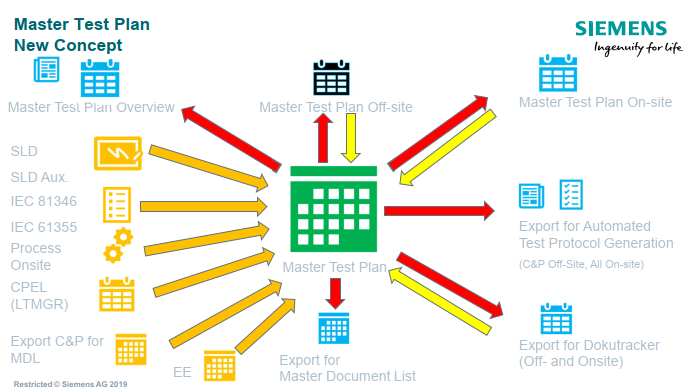
\includegraphics[width=0.9\textwidth]{Bilder/mtp} 
   \caption{Konzept des MTP, \cite{9}(S.2)} 
   \label{fig:struktur} 
   \end{center}
\end{figure}
%%
Er dient als Informationsursprung für weitere Dokumente und Arbeitsschritte im Laufe der Projektabwicklung. Durch Importe aus Listen und Diagrammen, die vom Kunden zur Verfügung gestellt werden, soll die Basis des \ac{mtp} erzeugt  werden. Einige dieser Dokumente sind auch bei Abnahme der Anlage oder bei Auswahl der Bauteile dem Kunden vorzulegen.
%%
\subsection{Master Test Matrix}
\label{sub:mtm}
%%
Die \ac{mtm} beschreibt verschiedene Testfälle und Testbedingungen, welchen die Anlage sowohl on- als auch off-site unterzogen wird. 
Diese Systemtests der Anlage werden auch im \ac{mtp} dokumentiert.
%%
\section{Dokumentationsnormen IEC 61355, IEC 81346 und ihre Verwendung}
\label{sec:iec}
%%
Da genannte Normen äußerst umfangreich und tiefgreifend sind, aber nicht alle Informationen zum Bearbeiten des Themas benötigt werden, wird im folgenden nur auf die wichtigen Grundlagen eingegangen.
Folgendes ist eine Zusammenfassung der relevanten Informatinen aus \cite[Kapitel 1-5]{3}, \cite[Kapitel 1-5]{4}, \cite[Kapitel 1-4,6]{5} und Gedankenprotokollen aus Mitarbeitergesprächen.
Die Normen enthalten Aussagen und Regeln zur Klassifizierung von Objekten und Dokumentationen in Stationen für Verteilung und Übertragung elektrischer Energie. Gearbeitet wird grundsätzlich noch mit dem Stand der Normen aus dem Jahr 2009 (IEC 81346-1/2) bzw. 2008 (IEC 61355).
\subsection{IEC 81346}
\label{sub:81346}
Die Kennzeichnung nach IEC 81346 bietet gegenüber früher genormten Kennzeichnungen weitergehende Möglichkeiten mit entsprechendem Rationalisierungspotential.
In IEC 81346-1 kann nach Aspekten unterschieden werden, diese sind Produktaspekt, Ortsaspekt und Funktionsaspekt. Ein Aspekt beschreibt die Betrachtungsweise für das Objekt. Grundsätzlich sollte jedes Objekt nach Produktaspekt strukturiert werden. IEC 81346-1 strukturiert Objekte nach diesen Aspekten und lässt somit eine klare Anlagenzusammensetzung erkennen. 
IEC 81346-2 typisiert Objekte in unterschiedliche Klassen und Unterklassen. Diese kommen auch bei der Strukturierung zum Einsatz.
In \ac{hgü}-Projekten wird die Dokumentenkennezichnung nach obenstehenden Normen durchgeführt. Objektkennzeichen beschreibt im weiteren die Kennzeichnung nach IEC 81346-1 und IEC 81346-2, zusammengesetzt aus Referenzkennzeichen und Objekttyp.
\\
\\
\subsubsection{Referenzkennzeichen}
\label{sub:refref}
%%
Das Referenzkennzeichen besteht aus maximal acht Leveln, beginnend mit der Stationsnummer. Danach folgt optional eine \markss{tieferliegende} Komponente. 
Die Strukturierung erfolgt meist von oben nach unten (top-down) oder von unten nach oben (bottom-up). Die Regeln erlauben im Prinzip einen Wechsel des Aspekts zwischen den Untergliederungsstufen einer Struktur, was jedoch in der Praxis selten zur Anwendung kommt.
%%
\begin{figure}[H]
   \begin{center}
   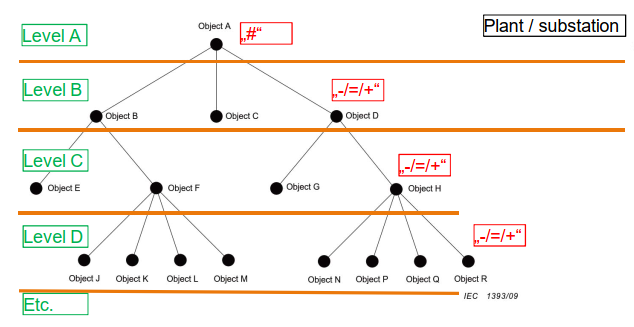
\includegraphics[width=0.9\textwidth]{Bilder/produktstruktur} 
   \caption{Struktur, \cite{10}(S.10)} 
   \label{fig:struktur} 
   \end{center}
\end{figure}
%%
Level A bezeichnet immer die Station, Level B und weitere beschreiben je eine durch einen Kennbuchstaben zugeordnete Funktion. Die Kennbuchstaben sind in der Norm tabellarisch festgehalten.
Einige Kennbuchstaben haben zusätzliche Unterklassen, um die Funkttion zu präzisieren. Sie werden durch zweistellige Kennbuchstaben definiert.
Die Kennbuchstaben der Strukturebene B und C sowie Darunterliegende unterscheiden sich grundsätzlich. Level B beschreibt Infrastrukturklassen, wie z.B. Umspannanlagen durch den Kennbuchstaben \markss{T}, während Level C und alle darunter Liegenden eine Klassifizierung nach Zweck oder Aufgabe beschreiben, z.B. definiert \markss{KF} die Funktion \markss{Verarbeiteung von elektrischen und elektronischen Signalen}.  
Der Übergang in das nächst niedrigere Level wird durch ein Trennzeichen dargestellt . Bei einem Funktionssaspekt wäre der Seperator \markss{=}, bei einem Ortsaspekt \markss{+} und bei einem Produktaspekt \markss{-}.
Erlaubt ist jedoch auch die Schreibweise \markss{-A1B1C1} oder \markss{-A1.B1.C1} statt \markss{-A1-B1-C1}.\\
Normalerweise wird jedes Objekt bei Siemens angesichts des Produktaspekt strukturiert. \\
Jedes Referenzkennzeichen ist laut Norm einzigartig.
\newpage
%%
\subsubsection{Objekttyp}
\label{sub:objektt}
%%
Der Objekttyp bedient sich den selben Objektklassen wie Strukturevel C des Referenzkennzeichens.\\
\markss{Alle Objekttypen, die bei “Transmission Systems” verwendet werden, sind im \ac{otc} enthalten.} \cite{5}(S.16) \\
Intern wird das Kürzel \ac{otc} stellvertretend für die Objektklasse verwendet, ist vom OTC die Rede ist eigentlich die Objektklasse mit allen fünf Stellen gemeint.
Alle Objekttypen sind wie folgt aufgebaut.
%%
\begin{figure}[H]
   \begin{center}
   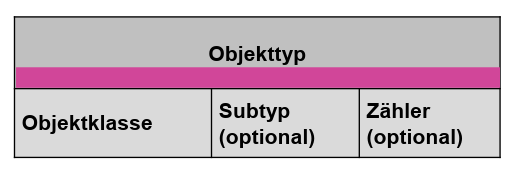
\includegraphics[width=0.9\textwidth]{Bilder/objekttypaufbau} 
   \caption{Zusammensetzung des Objekttyps, \cite{5}(S.18)} 
   \label{fig:objekttypaufbau} 
   \end{center}
\end{figure}
%%


%%
Bei der Bildung des Objekttyps wird unterschieden in physikalische und nicht-physikalische Objekte. \\
Nicht-physikalische Objekte behandeln Dokumente die keinem Produkt und keinem Ort eindeutig zugeordnet sind oder übergeordnet der Gesamtanlage dienen. Das sind z.B. Studien oder Projektmanagmentdokumente. Nicht-physikalische Objekte werden nur durch den Objekttypen gekennzeichnet. Sie haben kein Referenzkennzeichen. Nicht-physikalische Objektklassen werden durch fünf Zahlen gebildet, während physikalische Objektklassen aus zwei Buchstaben gefolgt von drei Zahlen bestehen.\\
Nicht physikalische Objekte sind in aktueller Ausarbeitung noch duch Siemens definiert. Der Zahlencode der physikalischen Objekte wird ebenfalls durch Siemens definiert, die Norm gibt nur den Buchstabencode vor.
Die Buchstaben entsprechen wie oben genannt dem Objektklassen-Code aus IEC8136-2.\\
Man erkennt in untenstehender Grafik deutlich, dass die Betrachtung des Objektes durch anhängen von drei Zahlen spezifiert wird.\\
%%
\begin{figure}[H]
   \begin{center}
   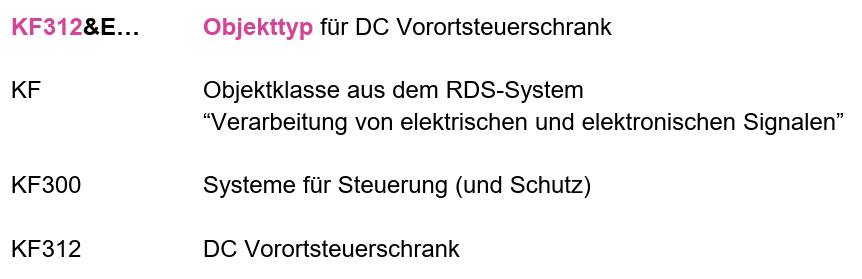
\includegraphics[width=1\textwidth]{Bilder/objekttyp} 
   \caption{Struktur eines physikalischen Objekttyps, \cite{5}(S.26)} 
   \label{fig:objekttyp} 
   \end{center}
\end{figure}
\newpage
%%
\subsubsection{Objektkennzeichen}
%%
Nachfolgende Grafik veranschaulicht die Kombination eines physikalischen Objekttyps und des Referenzkennzeichens nach Produktaspekt zum Objektkennzeichen.
%%
\pic{zusammen}{1}{Objektkennzeichen am Beispiel eines DC-Vorsteuerungsschrankes, \cite{5}(S.27)}{objektkennzeichen}
\newpage
%
\subsection{IEC 61355}
\label{sub:61355}
%
IEC 61355 erlaubt eine klar strukturierte Dokumentation zusammenhängend mit der eigenlichen Anlagenstruktur.
In der untenstehenden Grafik sieht man die Zusammensetzung der Normen zum Dokumentenkennzeichen bzw. Dokuemnetenseitenkennzeichen.
%%
\begin{figure}[H]
   \begin{center}
   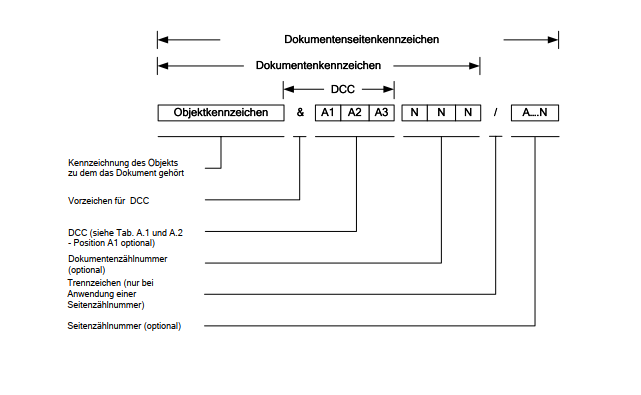
\includegraphics[width=1.1\textwidth]{Bilder/dokukennzeichen} 
   \caption{Dokumentenkennzeichnung, \cite{4}(S.12)} 
   \label{fig:dokk} 
   \end{center}
\end{figure}
%%
Wichtigster Bestandteil dieser Norm ist der \ac{dcc}.\\
Wie man in obiger Abbildung sieht, besteht der \ac{dcc} aus einem Vorzeichen, einem folgenden Kennbuchstaben, der den technischen Bereich des Dokuments bezeichnet und einem zweistelligen Buchstabencode, der die Dokumentenartklasse beschreibt. Die optionale Dokumentenzählnummer spezifiziert das Dokument. Der \ac{mtp} beinhaltet keinen \ac{dcc} ohne Dokumentenzählnummer. So beschreibt \markss{\&EFS010} einen dem Bereich Elektrotechnik (einschließlich Steuerungs-, Informations- und Kommunikationstechnik) zugeordneten Stromlaufplan. Das Kürzel \markss{FS} beschreibt übergeordnet Schaltkreisdokumente , während der Zahlencode \markss{010} auf Stromlaufplan spezifiziert.
Optional können noch Seitenzahlen angegeben werden.\\
Alle physischen Objekte, auch \markss{Equipment} genannt, bei Siemens folgen einer in \cite[S.47]{12} festgelegten Logik, nach welcher über jedes Objekt, übergeordnet eingteilt in Leittechnik- und nicht Leittechnik-Objekt, \markss{on-site} und \markss{off-site}, immer die selben Dokumentationen geführt werden müssen. Das komplette relevante Schema ist in Anhang \ref{sec:schema} zu sehen.
%%
\subsection{Dokumentennummer}
\label{sub:dokunummer}
%%
Die Anwendung beider Normen findet sich in der Bildung der Dokumentennummer wieder. Diese wird benötigt um alle Dokumente verschiedenster Art eindeutig zu kennzeichnen. Unter dieser Identifikationsummer werden diese später angelegt.
\\
%%
\begin{figure}[H]
   \begin{center}
   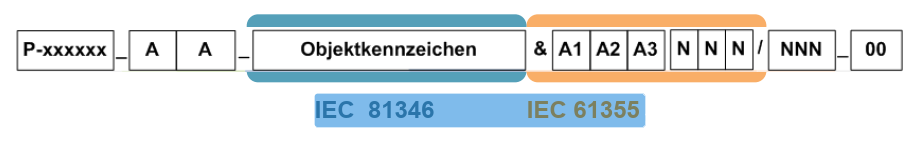
\includegraphics[width=0.9\textwidth]{Bilder/referenzkennzeichen} 
   \caption{Bildung der Dokumentennummer nach \cite{5}(S.8)} 
   \label{fig:doknum} 
   \end{center}
\end{figure}
%%

%%
Hinzu kommen hierbei noch der Projektcode, die zwei folgenden Kennbuchstaben und die Revisionsnummer an letzter Stelle. Der erste Kennbuchstabe beschreibt die Dokumentationsart, ob intern, extern oder Angebot, der zweite, den Aspektschlüssel aus Norm 81346-1.
\newpage
Der Aspektschlüsseltyp \markss{C}, der ein Objekt klassifiziert, das keinem anderen Aspektschlüssel zugewiesen werden kann, wird hier noch ergänzt. Das sind meist übergeordnete Dokumente zu mehreren Komponenten, z.B. Anlagenschaltpläne. Dieser ist nicht durch die Norm definiert, sondern intern. 
%%
\pic{aspectkey}{0.7}{Aspektschlüssel nach \cite{5}}{aspect}
%%
In der Grafik nicht sichtbar und auch in Norm bzw. interner Dokumentation nicht erwähnt, gliedert sich vor der Revisionsnummer noch das Sprachenkürzel für die Sprache des Dokuments ein.\\
Ein komplettes Beispiel einer Dokumentennummer ist \\
\inline{P-xxxxxx_EP_KF312#XY11-AF04-KF01-UH02&EFS010_EN_00}.
%%
\subsection{Dokumentendateiname}
\label{sub:dokudatei}
%%
Das Ablegen der Dokumente in den Projektverzeichnissen erfolgt durch einen der Dokumentennummer ähnlichen Dateinamen. Dieser wird aus der Dokumentennummer erzeugt, indem alle Trennzeichen durch \markss{\_} ersetzt werden. \markss{-}, \markss{+} und \markss{=} entfallen. Dadurch wird das Referenzkennzeichen als Block zusammengefasst. Die einzige Ausnahme besteht darin, dass das \markss{-} nach der Stationskennung zu einem \markss{\_} umgewandelt wird.\\
So ergibt sich \\
\inline{P-xxxxx_EP_KF312_XY11_AF04KF01UH02_EFS010_EN_00}.
%%
\newpage
\section{Polarion}
\label{sec:polarion}
%%
Wie einleitend genannt handelt es sich bei Polarion um ein browserbasiertes Tool, das Anforderungs-, Test- und Application-Lifecycle-Management, kurz ALM, liefert. \cite[vgl.]{1} \\
\markss{Polarion wird von globalen Unternehmen in einer Vielzahl von Branchen eingesetzt, wie zum Beispiel im Automobilbau, in der Medizintechnik und in der Luft- und Raumfahrt. Kunden erzielen mit Polarion die für die Herstellung Ihrer Produkte nötige Agilität, Traceability und Compliance. [...] Mehr als 2,5 Millionen Anwender weltweit vertrauen deswegen auf Polarion um die Zusammenarbeit in ihren Unternehmen voranzutreiben, ALM und Product Lifecycle Management (PLM) zu verknüpfen und um ihre hochwertigen Produkte auf den Markt zu bringen.} \cite{1} \\
Polarion läuft zentral auf einem Server, auf die der User per Browser zugreifen kann. \\
Die wichtigsten Funktion, die zur Implementierung dieser Arbeit dienen, werden folgend genannt. 
%%
\newpage
\subsection{Grundlegende Funktionalität}
\label{sub:funkti}
%%
In Polarion ist es möglich sogenannte Workitems einzupflegen, die an sich ein Objekt beschreiben. Dieses Objekt kann verschiedene Typen haben, dabei gibt es bereits fertige Standardtypen oder eigens erstellte \markss{Custom-Types}. Das Userinterface eines jeden Workitem-Types lässt sich durch erstellen neuer Felder bzw. das Umplatzieren dieser beliebig anpassen. 
Die in der Grafik erkennbare Kennung \markss{workitem-502} ist eine von Polarion selbst erzeugte ID, um jedes angelegte Workitem eindeutig zu kennzeichnen. Ein Ausschnitt der ganzen Benutzeroberfläche von Polarion ist im Anhang \ref{sec:polarionui} zu sehen. Darauf sieht man zusätzlich zur Grafik unten, noch das Fenster, in dem alle Workitems eines Typen aufgelistet werden. Diese Auflistung kann durch Abfragen verschiedener Parameter (Bilden von \markss{Queries}) manipuliert werden. Im Prinzip werden durch eine Query alle Workitems gefiltert und nach bestimmten Kriterien, z.B. dem Inhalt eines Feldes, gelistet. Die Poalrion-Query-Sprache ist grundsätzlich ähnlich zur Apache Lucene Syntax. \cite{13}
%%
\pic{testcase}{1}{Beispiel des Userinterface am Typen \markss{Test Case}}{testcase}
%%
Einige Felder des \ac{ui} sind bereits vordefiniert, meist werden sie vom System ausgefüllt, wie zum Beispiel das Feld \markss{Author}, und per default wie in Abbildung \ref{fig:testcase} zu sehen positionieren. Andere, sogenannte \markss{Custom-Fields} lassen sich per \ac{xml}-Datei anlegen und in einer auch als XML vorliegenden \markss{Form-Configuartion} im Interface anordnen. Es gibt viele unterschiedliche Custom-Field-Types, die häufigsten sind jedoch Enumeration und String.
\\
%%
\begin{figure}[H]
\begin{lstlisting}[language=XML]
<fields>
	<field description="Workitem Type" id="type" name="Type" type="enum:type"/>
	<field id="severity" name="Severity" type="enum:severity"/>
	<field id="author" name="Author" required="true" type="string"/>
	<field id="project" name="Project" type="string"/>
	<field id="categories" name="Categories" type="string"/>
<\fields>
\end{lstlisting}
\caption{Beispiel des Fields XML-Schema}
\label{fig:schema}
\end{figure} 
%%
Jede Felddefinition wird mit \inline{<field} begonnen und endet mit \inline{/>}. \inline{description} bezeichnet den in einer Pop-Up Box sichtbaren Text, wenn die Maus im UI über den Anzeigenamen des Feldes bewegt wird. \inline{name} beschreibt den Anzeigenamen des Feldes, \markss{id} den \ac{id} des Feldes und \inline{type} den Feldtypen.
Mit \inline{required="true"} wird festgelegt, welche Felder beim Anlegen eines einzelnen Items ausgefüllt sein müssen. Mit \inline{multi="true"} ist es möglich bei Feldern vom Typen \inline{enum} mehrere Optionen anzugeben.
Der Block der einzelnen Felder wird mit \inline{<fields>} begonnen und mit \inline{</fields>} beendet.
\newpage
%%
\begin{figure}[H]
\begin{lstlisting}[language=XML]
<!-- Horizontal layout element, adds components on horizontal row. Each component is in a new column. -->
    <horizontal>
        <!-- Vertical layout element adds components into one vertical column. Each component is in a new row. -->
        <vertical>
            <section>
                <field id="type" readOnly ="true" />
                <field id="severity" />
                <field id="author" />
                <field id="project" />
                <field id="categories" />
            </section>
 		  </vertical>
 	  </horizontal>
\end{lstlisting}
\caption{Beispiel des Form-Konfiguartion XML-Schema}
\label{fig:form}
\end{figure} 
%%
Wie im Beispielcode zu sehen beginnt \inline{<horizontal>} eine Reihe, \inline{<vertical>} eine Spalte und \inline{<section>} ein Element dieser Spalte. Wird ein Feld ohne Section definiert, so erscheint es als blauer Balken, wie \inline{Description} in Grafik \ref{fig:testcase}. 
Es gibt die Möglichkeit Felder mit \inline{readOnly="true"} nur lesbar zu setzen.
%%
Wenn ein Custom-Field als \markss{enum} definiert wird, muss in einem weiteren XML-Schema die Enumeration definiert werden. Enumerationen werden dann gewählt, wenn der Benutzer aus einem dropdown Listenfeld vorgegebene Werte auswählen soll. \\
%%
\begin{figure}[H]
\begin{lstlisting}[language=XML]
<enumeration>
	<option id="blocker" name="Blocker" description="" sortOrder="1"/>
	<option id="critical" name="Critical" description="" sortOrder="2"/>
	<option id="major" name="Major" description="" sortOrder="3"/>
	<option id="normal" name="Normal" description="" sortOrder="4" default="true"/>
	<option id="minor" name="Minor" description="" sortOrder="5"/>
	<option id="trivial" name="Trivial" description="" " sortOrder="6"/>
</enumeration>
\end{lstlisting}
\caption{Beispiel des Enumeration XML-Schema \markss{Severity}}
\label{fig:enum}
\end{figure} 
%%
Jeder auswählbare Wert wird hier als \inline{option} aufgeführt. Über den ID kann später darauf zugegriffen werden, \inline{name} gibt den Anzeigenamen an und \inline{description}, wie auch oben, den Text in der Pop-Up Box, die angezeigt wird, sobald die Maus über eine Option bewegt wird.
\inline{sortOrder} beschreibt die Reihenfolge in der die Optionen in der Klappliste angezeigt werden.
\\

Zusätzlich zu oben genannten Features verfügt Polarion über eine Import\-Funktion aus Excel-Workbooks und den Excel-Roundtrip-Change Import, bei dem bestehende Datensätze zuerst aus Polarion exportiert werden, bearbeitet und wieder importiert werden. Exportieren ist in fast alle gängigen Anzeigeformate möglich.\\
Verschiedene Benutzerrechtegruppen lassen sich auch erstellen.\\
Außerdem lassen sich in Polarion unterschiedlche Workitems miteinander verlinken, was es möglich macht Baumstrukturen zu erstellen, oder einen reinen Dokumentennamen mit dem tatsächlichen Dokument in Beziehung zu stellen.
\\
%%
%%
\subsection{Wiki Pages und Velocity}
\label{sub:veloc}
%%
Wiki-Pages sind editierbare Dokumente, die zum Anzeigen von Daten, Objekten und Informationen dienen sollen. Diese Dokumente stehen für jedes Projekt in einem übergeordneten Verzeichnis zur Verfügung. Sie sind Workitemtyp-unabhängig. Ein einfaches Beispiel hierfür wäre die Anzeige aller Workitems die mit einem bestimmten Flag, z.B. \markss{eilig} versehen sind. Diese \markss{Pages} können mit der Java-basierten Template Engine \markss{Velocity} (\cite{6}[vgl.]) editiert werden. Die verwendete Sprache, genannt \ac{vtl} lässt sich komplett in geschriebenen Text integrieren und bietet einige, wenn auch eingeschränkte, Funktionalitäten.
Diese Sprache soll \markss{die einfachste, unkomplizierteste und sauberste Möglichkeit bieten, dynamische Inhalte in eine Webseite zu integrieren.} \cite{6}. \\
Zusätzlich dazu stehen einige Templates aus Polarion zur Verfügung, die die Anzeige von Datensätzen vereinfachen oder einfach nur die Möglichkeit bieten Bilder in die Wiki-Page zu integrieren.
\\
Ein Zugriff auf die Polarion \ac{api} ist über bereits in­s­tan­zi­ie­rte Objekte der Services möglich, die einen Einstiegspunkt in die API ermöglichen.\\
Polarion arbeitet nicht mit der aktuellsten Version der \ac{vtl}, sonder mit Version 1.4. \cite[vgl. S.8]{18}\\
Ein kurzes Code-Beispiel unter Verwendung der API befindet sich in Anhang \ref{sec:veloapi}.
 
%%
%%
\subsection{API}
\label{sub:api}
%%
Polarion verfügt über eine Java \ac{api}, mit der es möglich ist Workitems zu ändern, zu lesen und zu erstellen, Benutzer zu verwalten, nach Workitems zu filtern oder Projekte aufzulisten, nur um ein paar Funktionen zu nennen. Zur Verfügung stehen verschiedene Services, mit unterschiedlichen Funktionen, mit denen der Zugriff auf den Polarion Server ermöglicht wird. (\cite{17}[vgl.]) \\
Einige der wichtigsten sind laut \cite{17}(S.3):
\subsubsection{ISecurityService}
%%
Ein Einstiegspunkt für Authentifizierungs- und Autorisierungsaufgaben. Die Aufgabe dieses Services ist es, Benutzer zu verwalten, Rollen zu verteilen, Beziehungen und Rechte anzulegen.
%%
\subsubsection{ITrackerService}
%%
Dieser Service dient als Haupteinstiegspunkt um Workitems zu verwalten. Er ermöglicht das Suchen, Lesen, Erstellen, Modifizieren und das verlinken von Workitems.
%%
\subsubsection{ITransactionService}
%%
Durch diesen Service ist es möglich Änderungen am Repository persistent zu machen. 
%%
\subsubsection{IDataService}
%%
Mit diesem Service ist eine Verwaltung von Objekt-Historien möglich.
%%
\subsection{Extension FMC}
\label{sub:fmc}
%%
Informationen über die Funktionsweise des Plugins, wurden dessen öffentlich einsehbaren Quellcodes bzw. der Funktionsanleitung entnommen. (\cite{8})\\
Die zur Verfügung gestellten Server haben bereits eine Extension vorinstalliert, die es möglich macht eigens verfasste Skripte in JavaScript in den Polarion-Wokflow zu integrieren. In diesen kann eingeschränkt auf die API zugegriffen werden, es stehen nur Instanzen des aktuellen Workitems, des \markss{TrackerService} und eines Loggers zur Vefügung.\\
Das Plugin überschreibt die von Polarion aufgerufene \markss{invoke}-Funktion, falls der \markss{save}-Parameter gesetzt ist und lässt somit nach dem Speichern eines Workitems, das die \markss{invoke}-Funktion mit dem gesetzten \markss{save}-Parameter aufruft, die Ausführung von eigenem Code zu. Sobald die im Code verfügbare Variable \markss{returnvalue} über einen Inhalt verfügt, wird dem User eine Error-Message angezeigt, die diesen Inhalt darstellt. Das Speichern wird somit verhindert. \\
Ein einfaches Beispiel wäre z.B. eine Überprüfung auf das Einhalten eines Prozentsatzes. Eine Kombination aus drei Feldern soll einen Prozentsatz von 100\% ergeben, bei einer Ungleichheit zu 100\% soll ein Speichern nicht möglich sein.
%%
%%
\subsection{PAM}
\label{sub:pam}
%%
Folgende Informationen sind aus einem Gedächtnisprotokoll mit Hr. Paul-Heinz Esters. \ac{pam} ist ursprünglich konzipiert um Software automatisch aus Anlagen-Datensätzen zu generieren. In \ac{pam} sollen zukünftig alle anlagenbezogenen Daten, von Nenndaten bis zu den Referenzkennzeichen der Bauteile gesammelt werden. Statt \ac{pam} zur Parametrisierung von Software zu benutzen, wird \ac{pam} allerdings als Daten-Backbone verwendet. 
%%
\section{Stand der Technik}
\label{sec:stand}
%%
Aktuell werden die Datensätze des \ac{mtp} über eine Excel-Tabelle verwaltet. Auf ein bestehendes Template wird über verschiedene Informationszugänge von Hand der schlussendliche Datensatz aufgebaut. Dieser Ansatz ist zwar funktional, aber grundsätzlich unhandlich und ohne einsichtlichen Userworkflow. Zusätzlich ist kein ausreichender Schutz vor Datenverlust bei Mehrfachzugriff möglich. 
Zu Arbeiten mit Polarion gibt es aktuell ein Pilotprojekt, dass die \ac{mtm} behandelt, ähnlich wie der \ac{mtp} über Excel verwaltet wurde.





%
\chapter{Bedarfsanalyse}
\label{cha:bedarf}
%%
\thispagestyle{scrheadings}
\pagestyle{scrheadings}
%%
Das Ziel der Arbeit ist das Transferieren eines \ac{mtp} einer \ac{hgü}-Anlage in die Umgebung von Polarion.\\
Die Oberfläche soll der Excel-Tabelle ähneln und für den Anwender leicht zu bedienen sein.
Folgende Punkte sind zu berücksichtigen:
\begin{compactenum}[(i)]
 \item Hinterlegung eines Workflows im Tool (Zugriffsrechte auf verschiedene Phasen und Komponenten je nach Projektrolle) 
 \item Import- und Exportfunktionen aus dieser Datenbasis 
 \item Berücksichtigung der Dokumentationsvorgaben (Kapitel \ref{sec:iec})
 \item Definition der erforderlichen Variablen, Erstellen von Eingabemasken (UI)
 \item Integration eines Trackings über den Dokumentationsstand
 \end{compactenum}
Punkt (i) ist zu Beginn gedacht, wird jedoch während der Bearbeitung verworfen bzw. verschoben.
Wie in Kapitel \ref{sec:polarion} genannt, gehört eine Import-/Exportfunktion bereits zum Funktionsumfang von Polarion. Jedoch ist es notwendig Importmasken zu definieren.
Während der Bearbeitung kommt die Idee auf, einen auf den Regeln zum Dokumentationsschema in Kapitel \ref{sub:61355} basierenden Workitem-Multiplikationsalgorythmus zu erstellen.
%%
\chapter{Entwurf}
\label{cha:ent}
\thispagestyle{scrheadings}
%%
Bevor erste Ansätze enstehen, wurden intensive Einarbeitungsgespräche mit Betreuer Paul-Heinz Esters geführt, die dem Zweck dienten einen ersten groben Überblick der Thematiken zu erhalten. Daraufhin erfolgt wie einleitend genannt eine Einarbeitungs-  und Lernphase, durch mehrere Dokumente, Lernvideos und einem Admin-Key Training zu Polarion. Zusätzlich dazu werden Gespräche mit dem Kollegen Andoni Sainz Lopez geführt, die über die API und die Erweiterung aus Kapitel \ref{sub:fmc} informieren.\\
%%
\section{Grundelegender Arbeitsblauf}
\label{sec:ablauf}
Zu Beginn soll der Ablauf des Projekts festgelegt werden. Dazu gehörte das Erstellen eines Übergeordneten Workflow-Diagramms. Der entgültige Arbeitsablauf steht erst zu Ende des Projekts fest, wird jedoch hier aufgeführt. Aufgrund der COVID-19 Pandemie laufen viele Unternehmensabläufe erschwert ab, die Kommunikation ist eingeschränkt und Tagungen von Ausschüssen zur Besprechung von internen Standards finden nicht oder verspätet statt. Das führt zu Verspätungen von Datenstandards, die zur Festlegung des Arbeitsablaufs nötig sind.
Zudem ergibt sich die in Kapitel \ref{cha:bedarf} genannt die Idee zur \markss{Datensatz-Multiplikation} erst im Laufe der Bearbeitung.
Wie in \ref{sub:mtm} erläutert erfasst der \ac{mtp} abschließend auch die Testdokumente der Systemtests der \ac{mtm}. Da dieses Projekt, wie in Kapitel \ref{sec:stand} ausgeführt, allerdings noch nicht vollständig ausgereift ist, wird in der Implementierung nicht darauf geachtet.\\
Außerdem sind zu gewissen Zeitpunkten, hier nicht aufgeführte, Exporte in das \ac{dms} vorgesehen.
\newpage
Im Folgenden ist der Ablauf geschildert. Die Funktonsweise bzw. der Zweck der Skripte wird später erläutert.

%%
\pic{projectworkflow}{0.9}{Projekt-Ablaufdiagramm}{workflow}
%%
%%
\section{Gestaltung der Anwenderoberfläche}
\label{sec:gest}
%%
Die Anwenderoberfläche in Polarion soll der Exceloberfläche so ähnlich wie möglich sein, um dem Benutzer die Umstellung auf das neue Portal so einfach wie möglich zu machen.\\
Grundsätzlich bedarf es einem neuen Workitem Typ.
Die benötigten \markss{Custom Fields} werden auf Grundlage des Excel-\ac{mtp} geplant, für Felder, die mit vordefinierten Inhalten gefüllt sind, werden Enumerationen vorgesehen. Grundätzlich soll jedes Feld der Excel-Vorlage in die Polarion-Version übernommen werden. Je mehr Felder als Enumerationen konfiguriert werden können, desto einfacher ist es fehlerhafte Eingaben durch den Anwender zu vermeiden. Da viele Felder, vorallem projektspezifische, wie z.B. die Stationskennung, nicht vorhersehbar sind, werden diese als Typ \markss{string} konfiguriert.
Eine Form-Konfiguartion, nach Abbildung \ref{fig:form}, wird zuerst theoretisch überlegt und auf Papier erstellt.
%%
%%
\section{Import- und Exportmasken}
\label{sec:import}
%%
Da das schlussendliche Projekt aus einer Mehrzahl an Datenquellen zusammengesetzt wird, muss feststehen, welche Informationen aus dem jeweiligen Import benötigt werden.\\
Wie in Abbildung \ref{fig:workflow} zu sehen ist, gibt es aktuell zwei Datenquellen für das Aufsetzen eines jeden Projektes.
Aus der Excel-Vorlage des \ac{mtp} werden alle Items importiert, die den Aspect-Key Typ \markss{C} haben. Diese sind größtenteils für jedes Projekt gleich, sodass nur kleine Änderungen vorgenommen werden müssen. \\
Da der Aspektschlüsseltyp \markss{F} nie geführt wird, werden Typ \markss{P} und \markss{L} aus der in Kapitel \ref{sub:pam} erwähnten PAM-Datenbank importiert. Dadurch wird jedes physische Objekt ohne \ac{dcc} in den \ac{mtp} aufgenommen.
%%
\section{Javascript Skripte auf der Basis FMC Work Item Save}
\label{sec:javascripte}
%%
Um dem User das bedienen der Oberfläche zu vereinfachen wird mit Skripten des FMC-Einschubprogramms (Plugin), Kapitel \ref{sub:fmc}, gearbeitet. Diese \markss{bauen} z.B. die, aus Kapitel \ref{sub:dokunummer} und \ref{sub:dokudatei}, Dokumentennummern und Dokumentendateinamen aus den einzelnen Bestandteilen zusammen. Es sollen so wenig Daten wie möglich importiert werden müssen, um die Importmasken bzw. die Exportmasken aus \ac{pam} so klein wie möglich zu halten. Deshalb füllen die Skripte das Workitem mit Daten, die aus dem kleinst-möglichen Import gewonnen werden können.

%%
\section{Multiplikationsverfahren}
\label{sec:multi}
%%
Dieser Teil orientiert sich nach \ref{sub:61355}, Absatz 4.
Da die Datensätze der physischen Objekte (Aspektschlüsseltyp P und L) der Anlage durch den Import aus Kapitel \ref{sec:import} ohne DCC vorhanden sind, werden diese durch Vervielfältigung und Anhängen eines DCC zu vollwertigen Dokumenten-Datensätzen.
Für den Multiplikationsalgorythmus gibt es zwei Konzepte, eines in Velocity, eingebettet in einer Wiki-Page, das andere als Erweiterung zu Polarion, auf Basis eines bereits vorhandenen Beispiels. Das erste Konzept erweißt sich als unbrauchbar und wird verworfen. Der theoretischer Ansatz des grundlegenden Algorythmus bzw. Aufbaus der Routine der beiden ist identisch.\\
Grundsätzlich soll es möglich sein Informationen durch den Anwender zu übergeben.
%%
\chapter{Implementierung}
\label{cha:impl}
\thispagestyle{scrheadings}
%%
Sämtliche\*r XML/Code und die \ac{mtp}-Vorlage sind unter folgendem Link abrufbar: \url{https://drive.google.com/drive/folders/1iwP3RyE5f7-kjzPVVpHDW35wfNTYXkVT?usp=sharing}.
%%
\section{Workitem Testdocument}
\label{sec:testdocu}
%%
Die Implementierung der neuen Benutzerobefläche, um den \ac{mtp} nach Polarion zu überführen, setzt die Erstellung eines eigenen Workitemtypen und einiger XML-Schemas vorraus. \\
Der neue Workitemtyp \markss{testdocument} wurde in Polarion mit allen vom System vorgegebenen Feldern und Werten angelegt.
Statt wie ursprünglich geplant, wird nicht jedes Feld des Excel-Plans in Polarion übernommen, sondern nur die wichtigsten. Der Excel-Plan ist über einige Jahre entstanden und während einige Felder nicht mehr benötigt werden, sind andere mehrfach vorhanden oder werden durch Funktionalitäten von Polarion abgelöst. Diese werden bewusst nicht übernommen. Implementiert wurden insgesamt 60 \markss{Custom-Fields}, von denen vier allein für die spätere Formkonfiguration dienen.\\
Folgende Felder wurden erstellt, ausgenommen den oben genannten vier.
Zu allen, in den Augen des Verfassers nicht offensichtlich ersichtlichen Feldern, wird ein kurzer Absatz gesagt. Die Felder sind in sinnhaften Blöcken angeordnet.
\newpage
%
\begin{table}[H]
  \centering
  \begin{tabular}{c}
  \parbox{10cm}{
    \begin{compactitem}
  \item TestingSite, type=enum
	\item DMS Identifier, type=string
	\item VSC, type=enum
    \item LCC, type=enum
	\item Object Type, type=enum
	\item Serialnumber, type=string
\end{compactitem}}
  \end{tabular}\\
  \label{tab:first}
  \caption{Wichtigste Query Informationen}
\end{table}

%
Um später durch Bilden von Queries zwischen, in Kapitel \ref{sec:hgue} genannten, off-site und on-site Dokumenten unterscheiden zu können wird hier das Feld \markss{TestingSite} angelegt. Der \markss{\ac{dms}-Identifier} dient dazu um Objekte, bei späteren Exporten in das \ac{dms} eindeutig zu Kennzeichnen. Unter \markss{VSC} und \markss{LCC} wird festgehalten, ob ein Dokument für den jeweiligen Anlagentyp optional oder erforderlich ist. Bei Kennzeichnung mit optional, kann später durch den Benutzer entschieden werden, ob das Dokument entfernt wird, oder nicht.
Der \markss{Object Type} beschreibt, ob das Objekt physikalisch oder nicht-physikalisch ist. \\
\newpage
%
\begin{table}[H]
\begin{tabular}{ll}
 \parbox{7cm}{
 \begin{compactitem}
  \item Documentnumber, type=string
	\item Documentfilename, type=string
	\item Document Type, type=enum
    \item Aspect Key, type=enum
	\item OTC Code, type=string
    \item Subtype, type=string
    \item Station number, type=string
    \item Level B, type=string
    \item Level C, type=string
    \item Level D, type=string
 \end{compactitem}}
 &
 \parbox{7cm}{
 \begin{compactitem}
  \item Level E, type=string
    \item Level F, type=string
    \item Level G, type=string
    \item Level H, type=string
	\item Code Letter, type=enum
	\item DCC Class, type=enum
	\item Language, type=enum
	\item Page Counter, type=string
    \item Revision, type=string
    \item OTC.Subtype, type=enum
 \end{compactitem}}
 \end{tabular}
 \label{tab:second}
 \caption{Kennzeichen}
 \end{table}

%
Dieser Block implementiert die in Kapitel \ref{sec:iec} genannten, normgerechten Bausteine der Dokumentennummer bzw. des Dokumentendateinamen.
Die Projekt-ID wird übergeordnet für alle Workitems gleich angelegt, muss also hier nicht extra erzeugt werden. Für spätere Exporte wird das Feld \markss{OTC.Subtype} angelegt, dass den \ac{otc} und seinen optionalen Subtypen in einen String zusammenfasst.
\newpage
%
\begin{table}[H]
  \centering
  \begin{tabular}{c}
  \parbox{10cm}{
    \begin{compactitem}
 \item Station number, L, type=string
    \item Level B, L, type=string
    \item Level C, L, type=string
    \item Level D, L, type=string
    \item Level E, L, type=string
    \item Level F, L, type=string
    \item Level G, L, type=string
    \item Level H, L, type=string
\end{compactitem}}
  \end{tabular}
  \label{tab:third}
  \caption{Optionaler Location-Aspekt}
\end{table}
%
Die durch diesen Block erstellten Level des Referenzkennzeichens, dienen dazu, falls ein Objekt bereits durch den Aspekt \markss{P} beschrieben wird, hier zusätzlich optionale Informationen über die Lokation des Objekts angeben zu können. Das ist besonders auf der Baustelle hilfreich, da so das physische Gegenstück des Dokuments schneller gefunden werden kann.
Sollte der Aspekt des Dokuments bereits \markss{L} sein, entfallen diese Informationen. Logischerweise können diese Informationen erst auf der Anlage eingetragen werden können. 
%
\begin{table}[H]
  \centering
  \begin{tabular}{c}
  \parbox{10cm}{
   \begin{compactitem}
\item Documenttitle, type=string
    \item DCC description, type=string
\end{compactitem}}
  \end{tabular}
  \label{tab:fourth}
  \caption{Überschriften}
\end{table}
%
Diese zwei Felder werden durch die in Kapitel \ref{sec:javascripte} erwähnte Methodik mit den Beschreibungen der jeweiligen OTC bzw. DCC befüllt.
Die Beschreibung des OTC dient gleichzeitig als Dokumententitel.
\\
\newpage
%
\begin{table}[H]
  \centering
  \begin{tabular}{c}
  \parbox{10cm}{
   \begin{compactitem}
 \item Responsible Department, type=enum
	\item Responsible SubPM, type=enum
\end{compactitem}}
  \end{tabular}
  \label{tab:fifth}
  \caption{Abteilung}
\end{table}
%
Die Abteilungsbezeichnung aus Feld \markss{Responsible Department} kann durch einen Eintrag in Feld \markss{Responsible SubPM} noch spezifiziert werden.
\\
%
\begin{table}[H]
  \centering
  \begin{tabular}{c}
  \parbox{10cm}{
    \begin{compactitem}
  \item issued for information, type=enum
    \item issued for approval, type=enum
    \item issued for design, type=enum
    \item issued for manufacture, type=enum
    \item issued for construction, type=enum
    \item as built, type=enum
\end{compactitem}}
  \end{tabular}
  \label{tab:sixth}
  \caption{Dokumentenmerkmale (documentflags)}
\end{table}
%
Die Felder dieses Blocks beschreiben eine übergeordnete Thematik des Dokuments. Zum Beispiel werden Prüfbescheinigungen (\&* QC04*) immer als \markss{issued for information} gekennzeichnet, während bei Inbetriebsetzungsanleitungen (\&* DC03*) \markss{issued for approval} vermerkt wird. Dadurch können später die richtigen Queries gebildet bzw. dem Kunden die für ihn relevanten Dokumente zur Verfügung gestellt werden.
\\ 
%
\begin{table}[H]
  \centering
  \begin{tabular}{c}
  \parbox{10cm}{
    \begin{compactitem}
    \item Contact Person at Siemens, type=string
    \item Manufacturer, type=string
    \item Contact Person at Manufacturer, type=string
    \item Work Progress, type=enum
    \item Originator, type=string
    \item Due Date, type=date
    \item Review Status, type=enum
    \item Reviewer, type=string
    \item Due Date, type=date
    \item Approval Status, type=enum
    \item Approver, type=string
    \item Due Date, type=date
\end{compactitem}}
  \end{tabular}
  \label{tab:seventh}
  \caption{Verantwortliche}
\end{table}
%
Durch diese Custom-Fields sind größtenteils Ansprechpartner bzw. allgemein Personen von Interesse im Bezug auf dieses Objekt vermerkt. Das \markss{Work Progess} Enumeration-Feld erfüllt die Aufgabe den Fortschritt zu überwachen, indem sich mit eigens erstellten Icons verschiedene Fortschritte eintragen lassen (0\%,25\%,50\%,75\%,100\%).\\
\\
%
Zu fast allen hier als Typ \markss{enum} aufgeführten Feldern wurde eine gleichnamige Enumeration erstellt, außer für die jenigen, die nur mit \markss{ja} oder \markss{nein} anzuwählen waren. Für diese wurde ein einziges, immer wieder verwendetes, XML-Schema \markss{enum:yon} erstellt. Alle Enumerations folgen dem in Kapitel \ref{sub:funkti} gezeigten XML-Schema. Die Enumeration des DCC und OTC wurden aus den jeweiligen Listen entnommen, nach Schema aufbereitet und impotiert, sodass jeder Code bzw. seine Beschreibung (z.B. DC071 = Installationsanleitung) in Polarion enthalten ist. Der Option ID ist immer der jeweilige Code bestehenden aus Kleinbuchstaben und die Beschreibung der Inhalt der \markss{description} Variable. Jeder einzelne DCC bzw. OTC hat immer eine Beschreibung. \\
Die restlichen Enumerationen beinhalten alle grundsätzlich logische Optionen, die hier nicht gesondert aufgezählt werden. 
%%
\subsubsection{Form Konfiguartion}
\label{sub:formconfig}
%%
Die vier restlichen Custom-Fields wurden als Abschnittsüberschriften für die Form-Konfiguartion benutzt. Die Felder wurden möglichst übersichtlich und logisch angeordnet.
\\
Das formkonfigurierte Interface zum Workitem \markss{Testdocument} ist ab Anhang \ref{sec:testdocuinter} zu sehen. 
Alle Abschnitte ab \markss{Comments} sind standardmäßig bei allen Workitem-Types aufgeführt und werden deshalb nicht mit abgebildet.
%%
%%
\newpage
\section{JavaScript Skripte}
\label{ses:javascripts}
%%
Insgesamt werden acht Skripte verfasst, die gemäß der \markss{readme}-Datei der FMC-Erweiterung (\cite{8}) in einem übergeordneten Skript \markss{testdocument-pre-save.js} nach dem in der Grafik zu sehenden Ablaufdiagramm strukturiert werden.
%
\pic{scriptsrunning}{1}{Ablaufdiagramm des Skript-Worklfows}{skriptworkflow}
%
Nachfolgend wird zu jedem einzelnen Skript kurz dessen Grundfunktion erläutert.
%%
\subsubsection{not\_save\_wo\_requiredfields.js}
\label{sub:notsavewo}
%%
Es ist in Polarion zwar möglich, bestimmte Felder als \markss{required} zu setzen, d.h. beim Anlegen eines Workitems müssen diese Felder immer gesetzt sein, allerdings ist diese Funktionalität leicht umgänglich, da z.B. bei Importen nicht darauf geachtet wird. \\
Während der Bearbeitung und des Testing stellte sich heraus, dass polarion auch beim Import bzw. bei der Vorschau der importierten Daten, die für die Erweiterung notwendige \markss{invoke}-Funktion aufruft. \\
Dieses Skript setzt eingehend den \markss{default}-Wert der Dokumentensprache auf \markss{EN}, da auch hier die Polarion eigene Funktion zur \markss{default value}-Vergabe nicht funktioniert.\\
Danach wird geprüft, ob die, für die restlichen Skripte erforderlichen Felder \markss{OTC}, \markss{Aspect Key} und \markss{Document Type} gesetzt sind. Ist das nicht der Fall, wird der Boolean \markss{execute} auf \markss{false} gesetzt und somit die restlichen Skripte nicht ausgeführt.
Zusätzlich wird die Variable \markss{returnvalue} mit den fehlenden Daten beschrieben und anschließend dem Benutzer anhand einer, durch das Plugin erzeugter, Pop-Up Nachricht dargestellt.
%%
\subsubsection{otc\_subtype\_builder.js}
\label{sub:otcbuilder}
%%
Dieses Skript nimmt den Inhalt der als String importierten Felder \markss{OTC} und \markss{Subtype}, und setzt daraus das Enum \markss{OTC.Subtype} zusammen. Dadurch wird auch überprüft, ob die eingegebenen Strings zusammengesetzt einen logischen Wert ergeben. Ist das nicht der Fall, versucht die Methode (\cite{14}) das Feld zu setzen, wobei aber bei einem übergebenem Argument, dass nicht als \markss{Enum-Option} verfügbar ist, das Enum-Feld auf \markss{null} gesetzt wird. Falls das passiert wird \markss{returnvalue} mit einem Hinweis auf eine fehlerhafte Eingabe beschrieben.
%%
\subsubsection{docfile\_num\_builder.js}
\label{sub:docfilenum}
%%
Das Skript implementiert die in Kapitel \ref{sub:fmc} als beispiel genannte Funktion, die Dokumentennummer, sowie den Dokumentendateinamen, aus ihren Bausteinen zusammenzusetzen. Für die Bausteine des Referenzkennzeichens wird aus Performance-Gründen eine Schleife mit Abbruchbedingung verwendet. Da das Referenzkennzeichen niemals ein Hierachielevel auslässt, kann ab dem Nichtvorhandensein eines einzelnen Levels die Bildung des Referenzkennzeichens beendet werden.\\
Da nicht alle Bausteine String-Felder sind, kann auch nicht alles in einer Schleife realisiert werden. Um auf den Inhalt eines Enum-Feldes zuzugreifen, muss die Methode \markss{getName()} verwendet werden, welche bei String-Felder entfällt.\\
Das Ersetzen der Steuerzeichen, der zuerst generierten Dokumentennummer, nach Kapitel \ref{sub:docfilenum} erfolgt durch die JavaScript-Methode \markss{replace} (\cite{15}) mit einem regulären Ausdruck als Argument. Da jedoch an einer Stelle diese Logik außer Kraft tritt, werden Dokumentennummer, sowie Dokumentendateiname in zwei Blöcke unterteilt und schlussendlich mit dem Trennzeichen \markss{\-} bzw. \markss{\_} zusammengesetzt.
%%
\subsubsection{doc\_title\_from\_otc.js}
\label{sub:titleotc}
%%
Der als Enumeration angelegte OTC führt zu jeder \markss{Enum-Option} die Bezeichnung als \markss{decription} der Enum-Option mit.\\
Durch die API-Methode \markss{getProperty()} mit dem Argument \markss{description} kann die Beschreibung der aktuell gesetzten Option abgefragt werden. Diese wird dann als Inhalt des Feldes \markss{Documenttitle} gesetzt und für spätere Zwecke in der gloablen Variable \markss{doctitle} abgespeichert.
%%
\subsubsection{title\_set\_name.js}
\label{sub:titleset}
%%
\markss{title\_set\_name.js} kombiniert die Bezeichnung des OTC, abgespeichert in \markss{doctitle}, und die Dokumentennummer zu einem String und setzt diesen als Workitem-Titel.
Falls die Dokumentennummer leer ist, wird nur die Bezeichnung des OTC als Titel gesetzt.
Wenn im aktuellen Titel das Steuerwort \markss{skip} steht, wird kein neuer Titel gesetzt, sondern der Alte beibehalten.
%%
\subsubsection{dcc\_description\_setter.js}
\label{sub:dccdes}
%%
Dieses Skript funktioniert identisch zu \markss{doc\_title\_from\_otc.js}, mit dem Ziel das Feld \markss{DCC description} mit dem Inhalt der DCC-Beschreibung zu setzen. Ist der DCC leer, wird das Feld nicht gesetzt.
%%
\subsubsection{non\_physical.js}
\label{sub:physicl}
%%
Anhand des OTCs wird in diesem Skript das Feld \markss{Object Type} gesetzt.\\
Der OTC wird mit der JavaScript Methode \markss{search} (\cite{16}) und einem regulärem Ausdruck als Argument durchsucht
Fünf Zahlen als OTC beschreiben ein \markss{non-physical} Objekt, sobald er mit einem Buchstaben beginnt, ist der Objekt Typ \markss{physical}. 
%%
\subsubsection{issued.js}
\label{sub:issued}
%%
Durch dieses Skript werden die Felder aus Tabelle \ref{tab:sixth} gesetzt. Nach einer, mit dem Betreuer Paul-Heinz Esters erarbeiteten Logik, wird der \markss{Issue} des jeweiligen Dokuments gesetzt.\\
Zu Beginn werden alle Felder auf die Option \markss{no} gesetzt.\\
\markss{as built} erhalten alle Dokumente mit DCC \markss{QC05*}, wobei das Sternchen als Platzhalter dient.
\markss{QC08*},\markss{DC03*} und \markss{DC18*} sind \markss{issued for approval}, \markss{QC04*} und \markss{QC1**} \markss{issued for information}.
%%
\newpage
\section{Multiplizierungsalgorythmus}
\label{sec:algo}
%%
Der Sinn dieser Routine ist es, dem Benutzer bzw. Verwalter des MTP in Polarion, die Arbeit abzunehmen, grundsätzlich immer gleiche DCCs für physische Objekte der Anlage einzupflegen. Der Nutzer soll schlussendlich einen fast fertigen MTP vor sich haben, bei dem es nur noch einigen Änderungen, z.B. zusätzlicher oder weniger Dokumente, bedarf. 
%%
\subsection{Wiki Page mit Velocity}
\label{sub:wikivelo}
%%
Ein erster Ansatz wird auf Basis einer Wiki-Page mit der \ac{vtl} erstellt. Die begrenzten Möglichkeiten der bereits veralteten Version sorgen jedoch für Probleme, weswegen der Ansatz verworfen wird. Bei dem Versuch mit Velocity wurde außerdem auf eine Informationsübrgabe von außen verzichtet, Parameter wurden \markss{hardgecoded}.
Die Grundlage des ersten Ansatzes, der Algorythmus, kann ohne viel Portierungsarbeit für den zweiten Ansatz weiterverwendet werden.
%%
\newpage
\subsection{Plugin auf Basis des Beispiels \markss{Servlet}}
\label{sub:servlet}
%%
Zum Programmieren des Plugins wird die \ac{ide} \markss{Eclipse for Java Enterprise Developers} verwendet. Die Einrichtung der Entwicklungsumgebung wird der Anleitung aus \cite{17}(S.4) entnommen. Statt wie in der Anleitung beschrieben muss im Feld \markss{Runtime JRE} nach vorangehender Installation \markss{jre1.8.0\_241} statt \markss{jdk-11.0.2} gewählt werden.
%%
\subsubsection{Workitemtyp \markss{properties}}
\label{sub:propertieswi}
%%
Um dem User wie erwünscht die Möglichkeit zu geben, die Parameter des Vervielfältigungsalgorythmus zu verändern, wurde ein neuer Workitem-Typ \markss{properties} erstellt. Dieser beihaltet folgende Custom-Fields:
%%
\begin{compactitem}
 \item otcs for c\&p objects, type=string
 \item dccs list for non c\&p objects, type=string
 \item dcc list for c\&p objects, type=string
 \item project ids, type=string
 \item dcc count for offsite cp, type=integer
 \item dcc count for offsite noncp, type=integer
 \item optional items list c\&p, type=string
 \item optional items list non c\&p, type=string
\end{compactitem}
%%
Über diese Felder legt der Benutzer fest, welche OTCs ein Leittechnikobjekt (c\&p object) beschreiben, welche DCCs ein Leittechnikobjekt bzw. nicht-Leittechnikobjekt erhält, welche Projekte von der Vervielfältigung betroffen sein sollen, wie viele DCCs eines Leittechnikobjektes bzw. nicht-Leittechnikobjektes \markss{off-site} bzw. \markss{on-site} sind und welche DCCs nur optional sind.\\
In den beiden Integer-Feldern, wird die Anzahl der \markss{off-site}-DCCs gespeichert.
Diese werden in der späteren Routine zuerst abgearbeitet. Sind die in den Feldern gespeicherte Anzahl der DCCs abgearbeitet, sind alle folgenden Dokumente für \markss{on-site}.
Die Grundlage des Testprojektes, sind die Listen aus Anhang \ref{sec:schema}.
Somit lassen sich alle Felder außer \markss{otcs for c\&p objects} und \markss{project id} befüllen. \markss{project id} entält in diesem Fall nur den ID des Testprojekts. Aktuell ist nur ein Projekt in diesem Feld möglich.
Die Liste der OTCs die ein Leittechnikobjekt beschreiben wurde aus \cite{20} entnommen.
%%
\subsubsection{Beispielplugin \markss{Servlet}}
\label{sub:beispiel}
%%
Die Beispielerweiterung von Polarion selbst wird von \cite{17}(S.8) wie folgt beschrieben: \markss{This example allows you to create an extension for Wiki pages in form of creating a custom servlet to inform users, e.g. about statistics at the Home or
Dashboard. The result will be your own servlet with a title and body represented by \glq.jsp\grq{} page (written by you) emebedded into a Wiki page.}\\
Eine \glq.jsp\grq{}-Datei, \glq.jsp\grq{} steht für \markss{Java Server Pages}, ist eine \ac{html}-Datei, die zusätzlich \markss{Java}-Code enthält und somit dynamische Webseiten ermöglicht. \cite{21}[vgl.]
Die Klasse des Beispiels erweitert die Javaklasse \markss{HttpServlet} und überschreibt die Methoden \markss{doPost()} und \markss{doGet()}. Im Funktionsrumpf von \markss{doGet()} wird der Beispielcode ausgeführt, in \markss{doPost()} wird \markss{doGet()} aufgerufen. Am Ende der \markss{doGet()} Methode werden Informationen an die \glq.jsp\grq{} Datei übergeben. Durch den Aufruf dieser Datei mit \\ \inline{<iframe  width= 100\%  height=  200   src=/polarion/example/   frameborder=0 ></iframe>} \\ im Code der Wiki-Page wird der Inhalt der Datei  dargestellt. In der \glq.jsp\grq{}-Datei können sowohl HTML als auch Polarion-Makros verwendet werden. Diese Informationen können dem Quellcode der Erweiterung entnommen werden. Dieser ist nicht öffetnlcih zugänglich, ist jedoch im Verzeichnis jeder Poalrion-installation vorhanden.\\
Auf Basis dieser Erweiterung wird ein eigenes Plugin entwickelt, die  Grundfunktionen bleiben erhalten.
%%
\newpage
\subsubsection{Plugin \markss{WorkItemsMultiply}}
\label{sub:workitemmul}
%%
In folgendem Klassendiagramm sind die implementierten bzw. abgeänderten Klassen zu sehen. \markss{ServiceServlet} implementiert die selbe Grundfunktion wie die Klasse\markss{CurrentUserWorkloadServlet} des Beispiels, jedoch wurde der Code im \markss{doGet()} Funktionsrumpf verändert.\\
%%
\pic{classdiagramm}{0.85}{Klassendiagramm der \markss{WorkItemsMultiply} Erweiterung}{classdia}
%%
\newpage
Die Funktionweise der Erweiterung wird anhand der einzelnen Klassen kurz erläutert. Alle Funktionen der API-Klassen können im Verzeichnis unter \cite{19} gefunden  werden. Die Stringvariablen \markss{returnvalue} und \markss{returnvalue[0]} der beiden Klassen werden kontinuierlich mit Debug-Informationen bzw. anwenderrelevanten Daten gefüllt und durch HTML formatiert. Diese Daten werden durch einfaches Ausgeben eines kombinierten Strings in \markss{rendered.jsp} dem Benutzer dargestellt.
%%
\subsubsection{ServiceServlet}
\label{sub:serv}
%%
Die Basisklasse der Erweiterung basiert wie oben genannt auf der Klasse des Polarion-Beispiels.\\
Sämtlicher Code wird, wie auch in der Beispielklasse, in der \markss{doGet()} Methode der Klasse ausgeführt.
%%
\newpage
\subparagraph{doGet}
%%
Um den in der \glq.jsp\grq{} Seite dargestellten Text in richtiger Programmablaufreihenfolge darzustellen, wird des Öfteren der \markss{Getter} \markss{getReturnvalue} des \markss{WorkItemsMultiply}-Objekts aufgerufen, anders als dargestellt.\\
In Folgender Grafik wird \markss{Beenden} bewusst in Anführungszeichen dargestellt, da ein, durch \markss{return}, Beenden in diesem Fall nicht möglich ist.
Die Funktion wird dadurch beendet, dass Daten an die \glq.jsp\grq{}-Datei übergeben werden. Statt also zu beenden, werden durch \markss{if}-Anweisungen die Aufrufe der \markss{WorkItemsMultiply}-Funktionen verhindert und dementsprechende Informationen an \markss{rendered.jsp} übergeben. Auch der Aufruf der \markss{Multiply}-Funktion kann fehlschlagen, allerdings wird danach sowieso die \markss{doGet}-Funktion \markss{beendet}.
%%
\pic{doget}{0.93}{Ablaufdiagram der \markss{doGet}-Methode}{ablaufdoget}
%%
%%
\subsubsection{WorkItemsMultiply}
\label{sub:workitemsm}
%%
Im Konstruktor der Klasse werden die grundlegenden Klassenvariablen initialisiert.
%%
\paragraph{getDependencies}
%%
Sollte ein Feld des \markss{properties}-Workitems leer sein, gibt die Funktion ein \markss{false} zurück und \markss{doGet()} übergibt die Information, mit Verweis auf das erste leere Feld, an die \glq.jsp\grq{} Datei. Das Einlesen bzw. Speichern der Parameter der Felder wurde durch ein \markss{Enum} und eine \markss{EnumMap}. Das sorgt für kompakteren und übersichtlicheren Code.
%%
\pic{getdependencies}{0.9}{Ablaufdiagramm der \markss{getDependencies}-Methode}{ablaufgetdep}
%%
\newpage
\paragraph{Multiply}
%%
Die Vervielfältigungsalgorythmen für die zwei Arten von Objekten unterscheiden sich nur durch die Anzahl der DCCs, der Art der DCCs und der Optionalität.
Die in \markss{getDependencies} gespeicherten Parameterdaten werden je nach Objektart für die Routine genutzt.\\
Aktuell wird bei jedem Workitem das Feld \markss{Code Letter} auf die Option \markss{E} gesetzt.\\
Die Funktionen des \markss{TransactionService} können bei Fehlschlagen eine \markss{java.lang.Exception} werfen, die von der höheren Instanz \markss{ServiveServlet} gefangen und verarbeitet wird.
%
\pic{multiply}{0.7}{Ablaufdiagramm der \markss{Multiply}-Metode}{multiply}
%
\pic{algo}{0.9}{Ablaufdaigramm der Vervielfältigungsroutine, fallunabhängig}{algo}
%
\newpage
\subsubsection{\markss{rendered.jsp}}
\label{sub:jsp}
%%
In der hier verwendeten Java Server Page, wird nur das, aus \markss{ServiceServlet.doGet()} übergebene, \markss{Object}-Array angenommen, gecastet und als einfacher String ausgegeben.
Die Formatierung dieses Strings findet in den Klassenfunktionen selbst statt.
%%
\begin{figure}[H]
\begin{lstlisting}[language=Java]
<%@ page import="java.util.Collection" %>
<%@ page import="java.util.Iterator" %>
<%@ page import="com.polarion.alm.tracker.model.IWorkItem" %>

<%
	    Object[] info  = (Object[])request.getAttribute("properties");
		String display = (String) info[0];
%>
Return: <%=display%>
\end{lstlisting}
\caption{rendered.jsp}
\label{fig:jsp}
\end{figure}
%%
\newpage
\section{Importmasken}
\label{sec:importmask}
%%
Die Objekte der beiden Aspektschlüssel \markss{P} und \markss{L} sollen aus PAM importiert werden. Dafür muss eine Import/Export-Maske festgelegt werden. Aufgrund der JavaSkripte aus Kapitel \ref{sec:javascripte} und dem Plugin aus Kapitel \ref{sec:multi} kann der Import auf ein Minimum reduziert werden.
Folgende Informationen pro Objekt müssen aus PAM als Import zur Verfügung stehen.
\begin{compactitem}
	\item Projekt ID
	\item Seriennummer
	\item Dokument Typ
	\item Aspektschlüssel
	\item Referenzkennzeichen
	\item OTC mit optionalem Subtypen
	\item Hersteller
	\item zusätzliches optionales Ortskennzeichen
\end{compactitem}
%%
\section{Bedienungsanleitung}
\label{sec:bedien}
%%
Nach allen Tests und Rücksprachen mit dem Betreuer wird eine kurze Bedienungsanleitung zur Verwendung des neuen Workitemtyps und des Plugin angefertigt. Diese beinhaltet den Arbeitsablauf, die zu erledigenden Arbeitsschritte, die benötigten Importdaten und kurze Erklärungen zu Skripten und Plugin.
%%
\chapter{Tests}
\label{cha:tests}
%%
Das auf die Implementierung folgende Testen wird aufgrund von Covid-19 mit reiner \markss{Dummy-Data} durchgeführt.\\
Dafür wurden sechs, auf Basis der Excel-MTP Vorlage erstellte, Workitems durch die Importfunktion in das Polarion Projekt importiert. Um später das Plugin zu Testen, werden jeweils zwei Workitems jedes relevanten Aspektschlüssels importiert. Während des Imports sind neben einigen Grundparametern, wie ab welcher Excel-Zelle der Import beginnen soll, auch ein \markss{Mapping} festzulegen, d.h. vorallem bei Enum-Felder muss festgelegt werden, welche Option der Zelle in Excel der Option des Feldes in Polarion entspricht. Das Mapping kann in eine Konfiguration gespeichert, um so später nocheinmal verwendet zu werden. In Anhang \ref{sec:import} ist ein Teil des Mappings plus der Importvorschau zu sehen.\\
Um die Funktionalität der JavaScript-Skripte zu testen, werden die importierten Workitems abgeändert und gespeichtert. Zusätzlich werden einige Sonderfälle erzwungen, um bei der Implementierung vergessene Möglichkeiten zu überprüfen.\\
Nach dem Import und Testen der Daten wird durch Aufrufen einer Wiki-Page, mit der in Kapitel \ref{sub:beispiel} genannten Codezeile als Inhalt, das Plugin aufgerufen. Nach einiger Rechenzeit wird auf der Seite der Rückgabetext angezeigt.\\ 
Im Prinzip wurde der Arbeitsablauf nach Abbildung \ref{fig:workflow} getestet, nur ohne reale Importe.
%
\chapter{Ergebnisse}
\label{cha:erg}
%%
Während des Imports stellt sich heraus, dass die JavaScript-Skripte auch während Erzeugung der Vorschau abgearbeitet werden. Das erspart dem Anwender einige Mühen, da nicht der gesamte Import fehlschlägt, sondern lediglich die Bildung der Vorschau. So kann schnell entweder das \markss{Mapping} oder die Importdatei geändert werden. Schlägt der gesamte Import fehlschlagen, muss die Rückgabeinformation der Skripte einer unübersichtlchen \markss{log}-Datei entnommen werden.  
Zudem zeigt sich, dass Polarion verlangt, dass entweder Titel- oder Beschreibungsfeld bei einem Import angegeben werden müssen. Beide werden aber durch Skripte automatisch befüllt. So muss \markss{Dummy}-Information auf eines der beiden Felder \markss{gemappt} werden.\\
Die durch das Plugin neu erstellten Workitems können in der Polarionbenutzeroberfläche (Abbildung \ref{fig:polarionui} betrachetet werden. Workitems des Aspektschlüssels \markss{C} bleiben wie erwartet vom Plugin unberührt.
%%
\paragraph{Probleme}
\label{par:prob}
%%
Anders als in der Anleitung \cite{17}(S.5) konnte das eigens entwickelte Plugin nicht in die installierte Polarion Anwendung importiert werden. Das Plugin funktioniert nur dann, wenn Polarion durch die IDE, wie in \cite{17}(S.6) beschrieben, gestartet wird. Jedoch funktioniert auf diesem Weg die \markss{FMC}-Erweiterung nicht. Somit konnte nicht getestet werden, ob wie erwünscht, das Speichern eines Workitems im Code des Plugins auch eine Abarbeitung der JavaSkripte zur Folge hat.\\
Zugleich scheint das Testen des Plugins \markss{Datenleichen} zu erzeugen, die zwar in der Polarionoberfläche augenscheinlich vorhanden und durch API-Funktionen \markss{geqeued} werden können, aber bei Zugriff über beide Möglichkeiten einen Fehler erzeugen und
die Exception \\ \markss{com.polarion.platform.persistence.UnresolvableObjectException} werfen. Im Revisionsverzeichnis aller Datensätze in Polarion werden diese Workitems allerdings nicht angezeigt. Polarion verfügt über eine \markss{Mainteance}-Funktion um einige bekannte Fehler zu beheben, Chache zu leeren oder \markss{log}-Datein zu erzeugen. Diese Funktion behebt das Problem nicht.\\
Möglicherweise werden diese erzeugt, wenn Objekte, die im Plugin noch referenziert sind, über die Oberfläche gelöscht werden. Das ist während des Testens des Öfteren passiert. Durch \markss{null}-Setzen der Objektreferenzen im Plugin und dem darauffolgenden Anstoß des Java \markss{Garbage-Collector} wird versucht dieses Problem zu lösen. Da bis zu diesem Zeitpunkt schon unübersichtlich viele \markss{tote Workitems} enstehen, ist es unmöglich zu Sehen, ob dies das Problem löst. Vielleicht liegt das Problem auch an völlig anderer Stelle. Kollegen kannten diesen Fehler nicht und der Polarion-Support ist, trotz Siemens-Zugehörigkeit, kaum zu Erreichen. Die Fehlermeldung ist in Anhang \ref{sec:error} abgebildet.
%%
%
\chapter{Zusammenfassung und Ausblick}
\label{cha:zusammenfassung}
\thispagestyle{scrheadings}
%
\hyphenation{} %% if the "compiler" does not seperate the word correctly, u can manually seperate words inside the brackets
%%
%\thispagestyle{scrheadings}
%\pagestyle{scrheadings}
%
\newpage
\addtocontents{toc}{\cftpagenumbersoff{chapter}}
%\newgeometry{left=35mm, right=35mm, top=35mm, bottom=35mm}
\bibliography{literatur}
\thispagestyle{empty}
\restoregeometry
\addtocontents{toc}{\cftpagenumberson{chapter}}
% 
\appendix
\pagenumbering{roman}
\newgeometry{left=35mm, right=35mm, top=20mm, bottom=20mm}
%%%
\chapter{Anhang}
%
\thispagestyle{empty}
\pagestyle{empty}
%%
\begin{landscape}
\section{Dokumentationsschema nach \cite{12}(S.47-50)}
\label{sec:schema}
%%
%%
\pic{schema1}{1.5}{Schema zur Dokumentation für Leittechnik Objekte off-site}{schema1}
\pic{schema2}{1.5}{Schema zur Dokumentation für Leittechnik Objekte on-site}{schema2}
\pic{schema3}{1.5}{Schema zur Dokumentation für nicht-Leittechnik Objekte off-site}{schema3}
\pic{schema4}{1.5}{Schema zur Dokumentation für nicht-Leittechnik Objekte on-site}{schema4}
%%
\section{Polarion-Oberfläche}
\label{sec:polarionui}
%%
\pic{polarion}{1.5}{Gesamte Benutzeroberfläche}{polarionui}
%%
\end{landscape}
%%
\section{Velocity und API Code-Beispiel}
\label{sec:veloapi}
%%
\begin{figure}[H]
\begin{lstlisting}[language=Java]
## 
## start transaction 
## 

$transactionService.beginTx() 
  
## 
## create a new workitem 
## 
#set($newWi=$trackerService.createWorkItem($projectService.getProject($page.project))) 
  
## set the workitem type 
#set($enumTypes=$trackerService.getTrackerProject($page.project).workItemTypeEnum) 
$newWi.setType($enumTypes.wrapOption("task")) 
  
## set the title 
$newWi.setTitle("Created by Velocity") 
  
## set the description 
#set($textObject=$objectFactory.newPlainText("This workitem was created by Velocity")) 
$newWi.setDescription($textObject) 
  
## save the workitem 
$newWi.save() 
  
## 
## end transaction, persist the work item changes 
## 
$transactionService.commitTx()
\end{lstlisting}
\caption{Codebeispiel Velocity}
\label{fig:bspvelo}
\end{figure} 
%%
Mit \inline{\#set()} werden Variablen gesetzt. Um eine Änderung an Workitems persistent zu machen, muss immer eine \inline{transaction} begonnen und nach dem Speichern des Workitems beendet werden.\\
Die Extension um die Instanz \inline{$objectFactory} zu verwenden, ist unter der verwendeten Polarionversion nicht mehr verfügbar.
%%
\section{Interface Testdocument}
\label{sec:testdocuinter}
\FloatBarrier
%%
 
\pic{workitem-405-1}{1}{Testdocument Teil 1}{testdocument1}
\newpage
%%
\pic{workitem-405-2}{1}{Testdocument Teil 2}{testdocument2}
%%
\begin{landscape}
\section{Importpreview}
\label{sec:import}
%%
\pic{preview}{1.8}{Preview eines Imports}{preview}
%%
\end{landscape}
\section{Fehlermeldung bei fehlerhaften Workitems}
\label{sec:error}
%%
\pic{error}{1}{Fehlermeldung/Exceptionstack}{error}
%%

%\unappendix
%end of appendix
\restoregeometry
%
\backmatter
%
\end{document}